% !Mode:: "TeX:UTF-8"
%\documentclass[fontset=mac]{ctexbeamer}
\documentclass[13pt, punct]{ctexbeamer}
\usefonttheme{professionalfonts}   % 数学公式字体
\usepackage{ctex}
\titlegraphic{
\includegraphics[width=2cm]{tjnu.jpg}}

\usepackage{color}
%\lineskip=9pt
\linespread{1.3}\selectfont
\makeatletter
\renewcommand\normalsize{%
	\@setfontsize\normalsize\@xpt\@xiipt
	\abovedisplayskip 1\p@ \@plus1\p@ \@minus6\p@
	\abovedisplayshortskip \z@ \@plus3\p@
	\belowdisplayshortskip 3\p@ \@plus3\p@ \@minus3\p@
	\belowdisplayskip \abovedisplayskip
	\let\@listi\@listI}
\makeatother
\parskip=6pt
%\usepackage{ctex}
%\usepackage[UTF8, heading = false, scheme = plain]{ctex}
%%%=== theme ===%%%
\usetheme{Madrid}
\useinnertheme{circles}
\setbeamertemplate{navigation symbols}{}
%\setbeamertemplate{footline}[page number]
\setbeamertemplate{footline}[frame number]{}



%\usepackage[style=numeric-comp, backend=bibtex, isbn=false, doi=false, url=false, eprint=false]{biblatex}
%\bibliography{../../../ref.bib}


\usepackage{lmodern}
\usepackage{amsmath}
\usepackage{amssymb}
\usepackage{latexsym}
\usepackage{amsthm}
\usepackage{mathrsfs}
%\usepackage{enumitem}
%\usepackage{enumerate}

%\usepackage{enumitem}
%\usepackage[colorlinks,
%            linkcolor=red,
%            anchorcolor=blue,
%            citecolor=green]{hyperref}
%%%%%%%%%%%%%%%%%%%%%%%%%%%%%%%%%%%%%

%%%%%%%%%%%%%%%%%%%%%%%%%%%%%%%%


\setbeamertemplate{theorems}[numbered]
\newtheorem{thm}{定理}[section]
\newtheorem{prop}[thm]{命题}
\newtheorem{cor}[thm]{推论}
\newtheorem{defi}[thm]{定义}
\newtheorem{lem}[thm]{引理}

\newtheorem{quest}[thm]{问题}
%\newtheorem{ex}[thm]{习题}
\newtheorem{conj}[thm]{猜想}

\def\sol{\noindent {\bf 解\ }}

\newtheorem{ex}{例}[section]

\definecolor{blue}{rgb}{0,0.08,1}
\newcommand{\blue}{\textcolor{blue}}





\begin{document}

\title{组\ 合\ 数\ 学}

\author{张\ 彪}
\institute[数学科学学院]{\normalsize 天津师范大学}
%\date[2011年10月13日]{\small 2011年10月13日}
\date[]{zhang@tjnu.edu.cn}

\frame[plain]{\titlepage}

\begin{frame}{第$2$章\quad 排列与组合}
\tableofcontents
\end{frame}


\AtBeginSection[]
{
	\begin{frame}
	\frametitle{排列与组合}
	\tableofcontents[currentsection]
\end{frame}
}

\section{加法原理与乘法原理}

\begin{frame}{加法原理}
	以下假设$A$和$B$是两类不同的、互不关联的事件。

\begin{thm}
	设事件$A$有$m$种选取方式,事件$B$有$n$种选取方式,则

	选$A$或$B$共有$m+n$种方式。
\end{thm}
\pause
		用集合的语言可将加法原理叙述成以下定理:
\begin{thm}
	设$A$, $B$为有限集,$A\cap B=\varnothing$, 则
	$$|A\cup B|=|A|+|B|.$$
\end{thm}
\end{frame}

\begin{frame}
\begin{ex}
从北京到上海可以乘飞机(3种方案),或者火车(5种方案)。

问从北京到上海共几种方案?


\end{ex}

\end{frame}

\begin{frame}\frametitle{乘法原理}

\begin{thm}
	设事件$A$有$m$种选取方式,事件$B$有$n$种选取方式,那么

	选取$A$以后再选取$B$共有$m\cdot n$种方式。
\end{thm}
\pause
用集合论的语言可将上述乘法原理叙述成如下的定理:
	\begin{thm}
		设$A,\ B$是两个有限集合,$|A|=m,\ |B|=n,$ 则
		$$|A\times B|=|A|\times|B|=m\cdot n.$$
	\end{thm}

\end{frame}

\begin{frame}
\begin{ex}
	从北京到上海有2条路线,从上海到深圳有5条路线。

	问从北京出发经由上海到深圳会有多少种路线?
\end{ex}

\begin{ex}
	求1400的不同的正因子个数。
\end{ex}
\pause
	$1400=2^3 \times 5^2 \times 7^1$

正因子为:$2^i \times 5^j \times 7^k$,其中$0 \le i \le 3, 0 \le j \le 2, 0\le k\le 1$

共计 $(3+1)(2+1)(1+1)=24$
\end{frame}

\begin{frame}
\begin{ex}
	在0和10000之间有多少个整数恰好有一位数字是5?
\end{ex}
\pause
通过添加0,把所有的数都看成是四位数,例如6=0006。

假如第 $i$位数是5,则有$9\times 9 \times 9=729$种可能。

共计$4 \times 729=2916$
\end{frame}



\begin{frame}
\begin{ex}
	在1000和9999之间各位数字不同的奇数有多少个?
\end{ex}
\pause
\begin{center}
	\begin{tabular}{|c|c|c|c|c|}\hline
		数位& 千位&百位& 十位& 个位\\ \hline
		选择范围& 1-9 &0-9& 0-9& 13579\\ \hline
	\end{tabular}
\end{center}
\pause
选取顺序: \pause 个位$\rightarrow$ 千位$\rightarrow$ 百位$\rightarrow$十位

\pause
答案: $5\times 8 \times 8 \times 7=2240$
\end{frame}


\begin{frame}
\begin{ex}\label{exa:subset}
	令$S=\{x_1,x_2,\ldots,x_n\}$是一个具有$n$元素的集合,或简称\,\emph{$n$元集}。

	再令$2^S$表示$S$的所有子集组成的集合,称为{幂集}。	求$2^S$的基数?
\end{ex}

\pause
{解:} 令$$\{0,1\}^n=\{(\varepsilon_1,\varepsilon_2,\ldots,\varepsilon_n)
\colon \varepsilon_i=0\mbox{或}1\}.$$
因为每个$\varepsilon_i$有两种可能的取值,所以有$$\#\{0,1\}^n=2^n.$$
定义映射$\theta \colon 2^S\rightarrow \{0,1\}^n$为
$$\theta(T)=(\varepsilon_1,\varepsilon_2,\ldots,\varepsilon_n),$$
其中
\begin{displaymath}
\varepsilon_i=\left\{ \begin{array}{ll}
1, & \mbox{  若 }x_i\in T  \\
0, & \mbox{  若 }x_i\notin T.
\end{array} \right.
\end{displaymath}
容易看出$\theta$是一个双射. 于是,$\#2^S=2^n$.
\end{frame}



\section{集合的排列}

\begin{frame}\frametitle{集合的排列}
\begin{defi}
	给定某个含有不同的元素集合$S$,我们把它的元素排成一个线性序,使得每个元素恰好出现一次,
	叫做该集合的一个\alert{排列 (permutation)}。
\end{defi}

以$[n]$表示$n$个正整数构成的集合$\{1,2,\cdots,n\}$, 那么$[n]$上的一个排列可以看成是$[n]$到自身的
一个\alert{双射}。

对于一个排列,我们可以用一行
$$\pi=\pi_1\pi_2 \cdots \pi_n$$
来表示,其中$\pi_i$表示$i$的像。
\end{frame}

\begin{frame}
我们来看一下$n$元集合的排列的个数。

\begin{thm}
	$n$元集合上全部排列的个数为
	$$n\times (n-1) \times (n-2)\times \cdots \times 2\times 1=n!.$$
\end{thm}

注意,为方便起见,我们令$0!=1$.

\begin{ex}
集合$[3]$上的排列个数为$3!=6$,它们分别为
	\[ 1\,2\,3,~~ 1\,3\,2,~~2\,1\,3,~~2\,3\,1,~~ 3\,1\,2,~~ 3\,2\,1.\]
\end{ex}
\end{frame}


\begin{frame}

\begin{defi}
	令$r$为正整数,从含有$n$个元素的集合$S$中取出$r$个元素排成一个线性序,叫做一个\alert{$r$-排列}。
\end{defi}

\pause

\begin{ex}
集合$[3]=\{1,2,3\}$上的$1$-排列为 \pause	$$1,~~2,~~3,$$
\pause	$2$-排列为   \pause	$$12,~~13,~~21,~~23,~~31,~~32.$$
\end{ex}
\end{frame}

\begin{frame}
用$P(n,r)$表示$n$元集合的$r$-排列的数目。

如果$r>n$, 则$P(n,r)=0$。

\begin{thm}
	对于正整数$n$和$r$, $r\leq n$, 有
	\[ P(n,r) = n \ (n-1) \cdots  (n-r+1).\]
\end{thm}
记$(n)_r=n \ (n-1) \cdots  (n-r+1)$,称为$n$的($r$阶)\alert{下阶乘}。

\end{frame}

\begin{frame}
    \begin{ex}
将$a, b, c, d, e, f$ 进行排列,问:

(1) 使得字母$b$ 正好在字母$e$ 左邻的排列有多少种?

(2) 使得字母$b$ 正好在字母$e$ 左边的排列有多少种?

    \end{ex}
    \pause

\end{frame}


\begin{frame}
\begin{ex}
从集合$\{1,2,\ldots,9\}$中取出7个不同的数字组成7位数,要求5和6不相邻,问有多少不同的种?

\end{ex}
\pause
所有的7位数
$P(9,7)=\frac{9!}{2!}=181440$

5和6相继出现的7位数
$P(7,5) \times  P(6,1) \times P(2,1) =\frac{7!}{2!}\times 6\times 2=30240$

共计  181440−30240=151200

\end{frame}


%\begin{frame}
%\begin{ex}
%	\begin{itemize}
%		\item[i)] 8对夫妇坐成一排,每对夫妇要坐在一起,则有多少种不同的坐法?
%
%		\item[ii)] 若围着圆桌坐,有多少种不同的坐法?
%	\end{itemize}
%\end{ex}
%\pause
% 答案: i) $8!$  \quad  ii) $7!$
%\end{frame}

\begin{frame}\frametitle{圆排列}

从$n$个不同的元素中取出$r$个元素排成一个圆环,按逆时针看去,完全相同这被认为是同一个\alert{圆排列}。
\begin{thm}
	$n$元集合的$r$-圆排列的个数为

	$$\frac{P(n,r)}{r}=\frac{n!}{r(n-r)!}.$$

	特别地, $n$元集合的圆排列是$(n-1)!.$
\end{thm}
\begin{ex}
10个人围坐一圈,其中有两人不愿挨着坐,问有多少种旋转排列方式?
\end{ex}
\pause
答案: $(10-1)! -2\times (9-1)!=282240.$
\end{frame}


\begin{frame}
\begin{ex}
	7个男生和3个女生聚餐,围坐在圆桌旁,任意两个女生不相邻。

	问有多少种旋转排列方式?
\end{ex}
\pause
答案: $(7-1)! \times P(7,3)=151200.$
\end{frame}


\begin{frame}
	\begin{ex}
	用7颗不同的珠子可以做成多少种不同的项链?
\end{ex}
\pause
答案:	$\frac{1}{2}(7-1)!=360$
\end{frame}
\begin{frame}
\begin{ex}
有4位同学各写一张贺卡,放在一起,然后每人从中取出一张,但不能取自己写的那一张贺卡。不同的取法有多少种?
\end{ex}
\pause
答案: $3!+3=9.$



提示:(错排问题)
把4位同学分别记为1,2,3,4, 假设第$i$位同学拿到了第$\pi_i$位同学写的贺卡,则$\pi_i \neq i$ 对于所有的 $1\le i  \le 4$.
于是,所求问题可以转化为求 排列满足
$\pi_1 \pi_2 \pi_3 \pi_4$, 其中$\pi_i \neq i$ 对于$1\le i  \le 4$
的个数.

然后,再考虑排列的圈表示,即求圈表示中不含1-圈的排列的个数.
\end{frame}


\begin{frame}
	\begin{ex}[m\' enage 问题]
		有4 对夫妇参加宴会围圆桌,要求男女相邻并且每对夫妇两人不得相邻,问有多少种就座方式?
	\end{ex}
	\pause
	答案:$(4-1)! \times 2 =  12$.


	提示:先让女士就座,就座方式有$(4-1)! =6$种,然后再让男士就座,只有2种可能.


%	然后再按照要求让男士就座,就座方式满足
%	$\pi_1 \pi_2 \pi_3 \pi_4$, 其中$\pi_i \neq i, i+1$对于 $1\le i  \le 3$ , 且 $\pi_4 \neq 1,4$.

%	只有两种可能,
\end{frame}
\section{集合的组合}
\begin{frame}\frametitle{集合的组合}
\begin{defi}
	$n$元集合的\alert{$k$-组合}是指从$S$中取出$k$个元素的一种无序选择,

	也可以看作是$S$的一个$k$元子集。
\end{defi}

\begin{ex}
若$S=\{a,b,c,d\}$,则 $$\{a,b\},\	\{a,c\},\ \{a,d\}, \ \{b,c\},\ \{b,d\},\ \{c,d\}$$
是$S$的所有$2$-组合。
\end{ex}
\end{frame}


\begin{frame}
用${n \choose k}$表示$n$元集合的$k$-组合的个数,读作“$n$取$k$”。




\pause
显然, 当$k>n$时,  ${n \choose k}=0.$
\begin{thm}
    若$0 \le k \le n$, 则
	$${n \choose k} = \frac{n (n-1) \cdots (n-k+1)}{k!}=\frac{n!}{k!(n-k)!}.$$
\end{thm}
$$n \ (n-1) \cdots (n-k+1) \overset{\alert{why?}}{=} {n \choose k} \cdot k!$$
\end{frame}

\begin{frame}
\begin{ex}
    系里欲将 6 名保送研究生推荐给 3 个单位,每个单位 2 名,问有多少种 方案?
\end{ex}


\begin{ex}
 { 从 } $1,2, \cdots, 100$ \text { 中选出两个不同的数,使其和为偶数, 问有多少种取法? }
\end{ex}



\end{frame}


\begin{frame}
\begin{ex}
在平面上给出25个点,任意三点不共线,这些点可以确定多少条直线?确定多少个三角形?
\end{ex}
\pause
两点确定一条直线 ${25 \choose 2} =300$,
\qquad
三点确定一个三角形 ${25 \choose 3} =2300$.


\begin{ex}在一个凸 $n(n \geqslant 4)$ 边形 $C$ 的内部, 如果没有三条对角线共点, 求其全 部对角线在 $C$ 内部的交点的个数.

\end{ex}
\end{frame}

\begin{frame}
\begin{ex}
如果要求每个``单词''包含3,4或5个元音字母,那么用26个英文字母可以构造多少个长度为8的``单词''?(字母使用次数无限制)


例如单词Andee使用了3个元音字母。
\end{ex}
\pause
3元音单词:$\binom{8}{3}\times 5^3 \times 21^5$,

4元音单词:$\binom{8}{4}\times 5^4 \times 21^4$,

5元音单词:$\binom{8}{5}\times 5^5 \times 21^3$,

共计:$\binom{8}{3}\times 5^3 \times 21^5 + \binom{8}{4}\times 5^4 \times 21^4 + \binom{8}{5}\times 5^5 \times 21^3$.

\end{frame}

\begin{frame}
    \begin{ex} 一个倶乐部有 10 名男成员和 12 名女成员, 现从中选出 4 人组成一个委员会, 若 要求:

(1) 至少要有 2 名女成员;

(2) 除 (1) 外, 又要求 $A$ 先生和 $B$ 女士不能同时入选。

分别求出有多少种不同的选法。
\end{ex}
\pause
解 (1) 设入选的女成员有 $i$ 名, 那么入选的男成员就有 $4-i$ 名, 其选法数为
$$
\left(\begin{array}{c}
    12 \\
    i
\end{array}\right)\left(\begin{array}{c}
    10 \\
    4-i
\end{array}\right)
$$
又 $2 \leqslant i \leqslant 4$, 所以选法总数为
$$
\left(\begin{array}{c}
    12 \\
    2
\end{array}\right)\left(\begin{array}{c}
    10 \\
    2
\end{array}\right)+\left(\begin{array}{c}
    12 \\
    3
\end{array}\right)\left(\begin{array}{c}
    10 \\
    1
\end{array}\right)+\left(\begin{array}{c}
    12 \\
    4
\end{array}\right)\left(\begin{array}{c}
    10 \\
    0
\end{array}\right)=5665
$$
\end{frame}

\begin{frame}
(2)从(1)中减去 $A$ 先生和 $B$ 女士同时入选的可能情况, 即为所求选法。

若 $A$ 先生和 $B$ 女士同时入选, 则另两名成员应从 9 名男士和 11 名女士中选出, 且至少选人一名女士, 与(1) 类似, 其选法数为
$$
\left(\begin{array}{c}
    11 \\
    2
\end{array}\right)\left(\begin{array}{l}
    9 \\
    0
\end{array}\right)+\left(\begin{array}{c}
    11 \\
    1
\end{array}\right)\left(\begin{array}{l}
    9 \\
    1
\end{array}\right)=99+55=154.
$$

因此, 共有 $5665-154=5511$ 种选法。


另法 \quad 总方案数 $=A, B$ 二人都不入选方案数 $+A$ 人选 $B$ 不入选方案数 $+A$ 不入选 $B$ 入选方案数, 即
总方案数为 $$ \sum_{i=2}^4\left(\begin{array}{c}11 \\ i\end{array}\right)\left(\begin{array}{c}9 \\ 4-i\end{array}\right)+\sum_{i=2}^3\left(\begin{array}{c}11 \\ i\end{array}\right)\left(\begin{array}{c}9 \\ 3-i\end{array}\right)+\sum_{i=1}^3\left(\begin{array}{c}11 \\ i\end{array}\right)\left(\begin{array}{c}9 \\ 3-i\end{array}\right)$$

\end{frame}

%\begin{frame}
%推论 \quad  若 $0 \leqslant r \leqslant n$, 则
%$$
%\left(\begin{array}{l}
%    n \\
%    r
%\end{array}\right)=\left(\begin{array}{c}
%    n \\
%    n-r
%\end{array}\right)
%$$
%
%
%
%定理 \quad 对任意正整数 $n$, 有
%$$
%\left(\begin{array}{l}
%    n \\
%    0
%\end{array}\right)+\left(\begin{array}{l}
%    n \\
%    1
%\end{array}\right)+\left(\begin{array}{l}
%    n \\
%    2
%\end{array}\right)+\cdots+\left(\begin{array}{l}
%    n \\
%    n
%\end{array}\right)=2^n
%$$
%\end{frame}



\section{多重集合的排列}
\begin{frame}\frametitle{多重集合的排列}


	\begin{ex}
		用3个A,2个B,4个C, 1个D可以构成多少个长度为10的字符串?
	\end{ex}
	\pause
%	$\displaystyle {10 \choose {3,2,4,1}}$
\alert{多重集}是元素可以重复出现的集合。

把某个元素$a_i$出现的次数$k_i$,叫做该元素的重数。

通常把含有$k$个不同元素的多重集$S$记做
$$\{ k_1 \cdot a_1, k_2 \cdot a_2, \ldots, k_n \cdot a_n \}$$
或者
$$\{ a_1^{k_1}, a_2^{k_2}, \ldots, a_k^{k_n} \}.$$
\end{frame}


\begin{frame}\frametitle{多重集合的排列}
用
$\Large{k_1+ k_2+k_n\choose k_1, k_2, \ldots, k_n}$
表示多重集合
$\{ k_1 \cdot a_1, k_2 \cdot a_2, \ldots, k_n \cdot a_n \}$的全排列个数。

先把$k_1+k_2+\cdots+k_n$个元素看成是互不相同的,

但这里$k_i$个$a_i$是相同的,只要两个排列中这些$a_i$的位置相同,就可以视为相同的多重集的排列。


\begin{thm}
$${k_1+k_2+\cdots+k_n \choose k_1, k_2, \ldots, k_n} = \frac{(k_1+k_2+\cdots+k_n)!}{k_1!k_2!\cdots k_n!}. $$
\end{thm}



\end{frame}


\begin{frame}
\begin{ex}
将单词MISSISSIPPI的字母重排,问有多少种排法?
\end{ex}

\pause
$\displaystyle {11 \choose {1,2,4,4}} = 34650$

\begin{ex}	将单词MISSISSIPPI的字母重排,要求不能出现连续的四个$S$,问有多少种排法?\end{ex}
\pause
$\displaystyle {11 \choose {1,2,4,4}}-{8 \choose {1,1,2,4}}=33810$

\end{frame}

\begin{frame}
\begin{ex}
	考虑\, 例\ref{exa:subset}\, 中定义的双射$\theta \colon 2^S\rightarrow \{0,1\}^n$。
	集合$S$上的\alert{$k$元子集} 与多重集$\{(n-k) \cdot 0, k \cdot 1\}$的排列一一对应。
\end{ex}

\pause $${n \choose k} = \frac{n!}{k!(n-k)!} = {n \choose n-k, k}$$
\end{frame}

\begin{frame}



\begin{ex}[格路计数问题]
在平面上有多少从 $(0,0)$ 到 $(m,n)\in \mathbb{N}\times\mathbb{N}$点的格路径,其每一步都

具有形式 $(1,0)$ 或 $(0,1)$ (即每一步向东或向北走一个单位距离)。
\end{ex}
    \begin{figure}
    \centering
    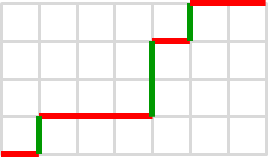
\includegraphics[scale=0.3]{path.png}
    \caption{格路}
\end{figure}

\pause

其与多重集$\{m \cdot E, n \cdot N\}$的排列一一对应。



\end{frame}


\begin{frame}
\begin{ex}
	从6男2女共8名学生中选出队长1人,副队长1人,普通队员2人组成4人服务队,要求服务队中至少有1名女生,共有多少种不同的选法?
\end{ex}
\pause
先选出4人:\quad 3男1女 \, 或 \, 2男2女

再考虑多重集合$\{1\cdot \mbox{队长}, \, 1 \cdot \mbox{副队长},\,  2 \cdot \mbox{普通队员} \}$的排列,比如
$$\left(\begin{array}{cccc}
\text{张三} & \text{李四} & \text{王五} & \text{赵六}\\
\text{队长} & \text{队员} & \text{副队长} & \text{队员}
\end{array}\right)$$


共计 $\big( {6 \choose 3} {2 \choose 1}  + {6 \choose 2} {2 \choose 2}  \big) \times {4 \choose 1,1,2}
= (40+15)\times 12 =660$.


该题来自2017年浙江高考。
\end{frame}


\begin{frame}
%    \frametitle{插空法}


\begin{ex}	在由四个$0$和八个$1$组成的序列$(a_1,a_2,\ldots,a_{12})$中,没有两个连续$0$的序列有多少个?
\end{ex}

\pause
{插空法} \quad $\displaystyle {8+1 \choose 4}=126$


%\begin{ex}
%	4个C和8个R的排列中没有两个C是相邻的,有多少种排法?
%\end{ex}

%\begin{ex}
%	用3个N, 3个S, 2个L, 5个E 以及A, H, V, I, T各一个,可组成多少个长度为18的字符串,使得第一个N在所有的S之后,并且T在第一个E之后?
%\end{ex}

\end{frame}

\begin{frame}
\begin{ex}
将 6 个蓝球、5个红球、4个白球、3个黄球排成一行,要求黄球不挨着, 问 有多少种排列方式?
\end{ex}
\pause
 先将蓝、红、白三种球进行全排列, 再将 3 个黄球揷 人其中.

 令 $M=\{6 \cdot b, 5 \cdot r, 4 \cdot w\}$, 则 $M$ 的全排列数为 $\frac{15 !}{6 ! 5 ! 4 !}$.

  每 个“*"表示 $M$ 的一个全排列中的一个元素, 共有 15 个 “*”,则可以在 16 个“ $\triangle$ ”所 示位置中选出 3 个插入 3 个黄球,共有 $ \binom{16}{3}$ 种取法.

  所以,共有 $\frac{15 !}{6 ! 5 ! 4 !} \cdot \binom{16}{3}$ 种排列方法.

\end{frame}


\section{多重集合的组合}


\begin{frame}
\begin{block}{引例}
    一家面包房生产8种炸面包圈。
如果将一打(12个)炸面包圈装进盒内,则一共有多少种不同的盒装组合?

\end{block}

\begin{block}{引例}
求
$$x_1+x_2+\cdots+x_n=r$$
的非负整数解的个数。
\end{block}

\begin{block}{引例}
将$r$个相同的小球放入$n$个不同的盒子中,要求每个盒子小球的个数不受限制,有多少种方法?
\end{block}

\end{frame}
\begin{frame}{多重集合的组合}
假定$n$个不同物体中的每一个都可以被重复选取任意多次。

用${n\choose
	r}\!\big)$表示从
$$\{\infty \cdot a_1, \infty \cdot a_2, \ldots, \infty \cdot a_n\}$$
选取基数为$r$的多重集的方法数。

设元素$a_i$出现$x_i$次。 该问题等价于求
$$x_1+x_2+\cdots+x_n=r$$
的非负整数解的个数。

这相当于,将$r$个相同的小球放入$n$个不同的箱子中
(即 将$r$个相同的小球排成一排,然后在小球中间插入$n-1$个隔板,隔板将小球分成了$n$份)

因此,原问题转化为多重集合$\{r \cdot \circ, (n-1) \cdot  | \}$的排列数。

所以,$\big(\!{n\choose r}\!\big)={n+r-1\choose r}$.
\end{frame}

\begin{frame}

\begin{ex}
	一家面包房生产8种炸面包圈。
	\begin{itemize}
		\item[i)]如果将一打(12个)炸面包圈装进盒内,则一共有多少种不同的盒装组合?

		\item[ii)] 若每盒必定包含所有的8种炸面包圈呢?
	\end{itemize}
\end{ex}
\pause  \qquad
i)  $\big(\!{8 \choose 12}\!\big)={12+8-1\choose 12}={19\choose 12}$, \qquad
ii) $\big(\!{8 \choose 4}\!\big)={12-1\choose 4}= {11 \choose 4}$
\end{frame}

\begin{frame}
	\begin{ex}
		方程$x_1+x_2+\dots +x_n=r$
		\begin{itemize}
			\item[i)]	非负整数解有多少个?

			\item[ii)] 	正整数解有多少个?
		\end{itemize}
	\end{ex}
	\pause

	i) $\big(\!{n\choose r}\!\big)={n+r-1\choose r}={n+r-1\choose n-1}$,

	ii) 法一:把$r$个相同的小球放入$n$个不同的盒子,要求每个盒子非空。
	这相当于,将$r$个相同的小球排成一列,然后在小球之间插入$n-1$个隔板  将小球分成了$n$份,每一份的数量都要大于或等于1 ,对应上述方程的一组正整数解。
	{\Large $$\circ \circ \circ |  \circ  \circ | \circ \circ \circ$$}
	也就是说,从$r-1$个位置挑出$n-1$个位置,用于放置隔板,即${r-1 \choose n-1}$。

	\quad 法二:令$y_i=x_i-1$, 则问题转化为方程$y_1+y_2+\dots +y_n=r-n$的非负整数解的个数,即 ${n+(r-n)-1 \choose r-n} = {r-1 \choose n-1}$.

\end{frame}




\begin{frame}
\begin{ex}
方程$$x_1+x_2+x_3+x_4=20$$的满足$$x_1\ge 4,  \,   x_2\ge 2,   \,  x_3\ge -1,  \,   x_4\ge 0$$的整数解有多少个?
\end{ex}
\pause
我们引入新变量
$y_1 = x_1-4,  \,  y_2 = x_2-2, \,  y_3 = x_3+1,  \,  y_4 = x_4$.

原问题变为方程
$$y_1 +y_2 +y_3 +y_4 = 15$$
的非负整数解的个数${4+15 -1 \choose 4-1}= {18 \choose 3}=816$.
\end{frame}


\begin{frame}\frametitle{Balls in boxes}
    I will tell you shamelessly what my bottom line is:
    \alert{It is placing balls into boxes}.
    \qquad	\qquad	\qquad	\qquad	 \qquad  ---\ \blue{Gian-Carlo Rota}, \emph{Indiscrete Thoughts}

    Gian-Carlo Rota was a math professor at MIT from 1959 until his death in 1999.
    He is arguably the father of the field today known as  combinatorics.

    \begin{ex}
        \begin{itemize}
            \item[i)]	将$r$个相同的小球放入$n$个不同的盒子中,有多少种方法?

            \item[ii)] 若要求每个盒子中至少有一个小球,有多少种方法?
        \end{itemize}
    \end{ex}

    \pause
    方程$x_1+x_2+\dots +x_n=r$
    \begin{itemize}
        \item[i)] 非负整数解

        \item[ii)] 正整数解
    \end{itemize}
\end{frame}


\begin{frame}
	对$\big(\!{n\choose	r}\!\big)={n+r-1\choose	r}$的一个直接的组合证明如下。

	令$$1\leq a_1< a_2<\cdots <a_r\leq n+r-1$$为$[n+r-1]$的一个$r$元子集。令$b_i=a_i-i+1$,则$\{b_1,b_2,\ldots,b_r\}$是$[n]$的一个$r$元重集。

	反之,给定$[n]$上的一个$r$元重集$$1\leq b_1\leq b_2\leq\cdots\leq b_r\leq
	n,$$定义$a_i=b_i+i-1$,则$\{a_1,a_2,\ldots,a_r\}$是$[n+r-1]$的$r$元子集。

	这样就定义了$[n]$的$r$元重集与$[n+r-1]$的$
	r$元子集之间的双射。
\end{frame}



\begin{frame}\frametitle{多重集合的组合数(有重数限制)}

令$$S= \{k_1 \cdot a_1, k_2 \cdot a_2, \ldots, k_n \cdot a_n\}$$是一个多重集,多重集合的$r$−组合数的计数问题更为困难。
等价于方程$$x_1+x_2+\cdots+x_n=r$$的整数解的个数,
其中$0\le x_1 \le k_1, \, 0\le x_2 \le k_2, \,  \ldots, \, 0\le x_n \le k_n$.

将在后面的课程中
%容斥原理或生成函数
解决该问题。

\end{frame}

%
%
%\begin{frame}\frametitle{有序分拆}
%\begin{ex}
%	$n$的一个\alert{有序分拆}(Composition)是指将$n$表示为一些{\em 有序}的正整数之和。例如$4$
%	有$8$个有序分拆,分别为
%	\[\begin{matrix}
%	1+1+1+1 & 3+1\\
%	2+1+1 & 1+3\\
%	1+2+1 & 2+2\\
%	1+1+2 & 4
%	\end{matrix}
%	\]
%
%	如果在一个有序分拆$\sigma$中有正好$k$个求和项,我们称$\sigma$有$k$个{\em
%		部分}并称$\sigma$为一个\alert{$k$-有序分拆}。\\[6pt]
%
%	问:$n$的{$k$-有序分拆}共有多少个?$n$的{有序分拆}共有多少个?
%\end{ex}
%
%\end{frame}
%
%\begin{frame}\frametitle{有序分拆}
%	给定$$(a_1, a_2, \ldots, a_k)$$
%	是$n$的一个$k$-有序分拆,定义$\theta(\sigma)$为$[n-1]$的一个$(k-1)$元子集:
%	\begin{displaymath}
%	\theta(\sigma)=\{a_1,a_1+a_2,\ldots,a_1+a_2+\cdots+a_{k-1}\}.
%	\end{displaymath}
%	反之,给定$$S=\{b_1, b_2, \ldots, b_{k-1}\}_{<}$$是$[n-1]$的一个$(k-1)$元子集,
%	定义$\phi(S)$为$n$的一个$k$-有序分拆:
%	\begin{displaymath}
%	\phi(S)=(b_1, b_2-b_1, \ldots, b_{k-1}-b_{k-2}, n-b_{k-1}).
%	\end{displaymath}
%	这给出了$n$的$k$-有序分拆到$[n-1]$的$(k-1)$元子集之间的一个双射。
%
%	因此,	一共有${n-1}\choose{k-1}$个$n$的$k$-有序分拆,而$n$的有序分拆个数为$2^{n-1}$。
%\end{frame}
%
%\begin{frame}\frametitle{有序分拆}
%	双射$\theta$常常以下面的图形表示:
%	将$n$个点画在一排,然后在$n-1$个分隔点的空位画$k-1$条竖直隔板。
%
%	这就将点分成了$k$个有序的“间隔”,其中每个部分含有点
%	的个数就构成了$n$的一个$k$-有序分拆。例如
%	{\Large $$ .\,|\,.\,.\,|\,.\,|\,.\,|\,.\,.\,.\,|\,.\,. $$ }
%	就对应有序分拆$$1+2+1+1+3+2$$
%
%\end{frame}

%
%\begin{frame}
%	一个与有序分拆紧密相连的问题是计数方程$x_1+x_2+\cdots+x_k=n$的非负整数解的个数$N(n,k)$。
%
%	这样的解称为将$n$分成$k$部分的一个{\em 弱有序分拆},或称$n$的{\em
%		弱$k$-有序分拆}。(正整数解就是$n$的$k$-有序分拆。)
%
%	如果我们令$y_i=x_i+1$, 则$N(n,k)$就是方程
%	$y_1+y_2+\cdots+y_k=n+k$的正整数解的个数,即$n+k$的$k$-有序分拆数。
%	于是有$N(n,k)={{n+k-1}\choose
%		{k-1}}$。
%
%	利用类似的方法可以证明方程$x_1+x_2+\cdots+x_k\leq
%	n$的非负整数解的个数为${n+k}\choose
%	{k}$。
%\end{frame}

%
%
%\begin{frame}\frametitle{集合划分}
%
%	若集合$A$的非空子集的集合
%	$$P=\{ A_1, A_2, \ldots, A_k \},$$
%	满足
%	$$A=\cup_{i=1}^k A_i, \quad \mbox{且} \quad A_i \cap A_j = \phi,$$
%	则称	$P$是集合$A$的一个\alert{划分}。
%
%	\begin{ex}
%	集合$[3]$划分成三个子集合的方法只有一种: $1/2/3$;
%	划分成两个子集合的方法有三种: $12/3,13/2,1/23$;
%	划分成一个子集合的方法只有一种: $123$.
%	\end{ex}
%
%令$S(n,k)$是$n$元集合的恰有$k$个部分的划分的个数。
%\end{frame}
%
%\begin{frame}
%\begin{ex}
%	把集合$\{1,2,\ldots,n\}$划分成$b_1$个1-子集,$b_2$个2-子集,$\dots$, $b_k$个$k$-子集,其中$\sum_{i=1}^k i b_i=n$,这样的分法有多少种?
%\end{ex}
%
%\begin{ex}
%	$S_n$中轮换型号为$(\ell_1,\ell_2,\ldots,\ell_n)$的排列共有多少个?
%\end{ex}
%\end{frame}
%
%
%
%
%\begin{frame}{Twelvefold way}
%
%下面的表格列出了各类不等价映射$f \colon N\rightarrow M$的个数,其中$|N|=n$而$|M|=m$。
%
%%\vskip 10pt
%%\noindent{\bf Twelvefold way}\\[-5pt]
%\rule{\textwidth}{1pt}
%\begin{tabular*}{\textwidth}{@{\extracolsep{\fill}}l|l||l|l|l}
%	$N$中元素	&	$M$中元素	&	$f$任意	&	$f$单射	&	$f$满射 \\
%	\hline & & & &  \\
%	可区分 & 可区分 & $^{1.}$ $m^n$ & $^{2.}$ $(m)_n$ & $^{3.}$ $m!S(n,m)$\\[5pt]
%	\hline & & & &  \\
%	不可区分 & 可区分 & $^{4.}$ ${m+n-1 \choose n}$ &
%	$^{5.}$ $m\choose n$ & $^{6.}$ ${n-1 \choose m-1}$\\[5pt]
%	\hline & & & &  \\
%	可区分 & 不可区分 & $^{7.}$ $\sum_{i=1}^{m}S(n,i)$ & $^{8.}$ $\delta (n\leq m)$ & $^{9.}$ $S(n,m)$\\[5pt]
%	\hline & & & &  \\
%	 不可区分 & 不可区分 & $^{10.}$ $\sum_{i=1}^{x}p_i(n)$ & $^{11.}$ $\delta (n\leq x)$ & $^{12.}$ $p_m(n)$
%\end{tabular*}
%\rule{\textwidth}{1pt}
%
%\end{frame}


\begin{frame}{补充题}



%我们从十二个简单的计数问题开始。
%找出下列各题尽可能简单的解答。
\begin{enumerate}
	\item  集合 $[10]=\{1,2,\ldots,10\}$ 有多少个至少包含一个奇数的子集?\\[8pt]

\item 将十个人分成五组,每组两人,不考虑分组顺序, 这样的分法有多少种?
	\item	计算满足 $\pi_1\neq 2$的6阶排列$\pi=\pi_1\pi_2\pi_3\pi_4\pi_5\pi_6$的个数。\\[8pt]

	\item	有多少个6阶排列恰好有两个圈?(不动点可以认为是长为1的圈)
\end{enumerate}

\pause
\begin{enumerate}
	\item $2^{10}-2^{5}=992$
	\item  $1\cdot3\cdot5\cdot7\cdot9=945$
	\item $5\cdot 5!=600$(或者$6!-5!=600$)
	\item $\displaystyle {6\choose 1}4!+{6\choose 2}3!+\frac{1}{2}{6\choose 3}2!^2=274$
\end{enumerate}
\end{frame}

\begin{frame}
	\begin{ex}
	把集合 $\{1,2, \ldots, n\}$ 划分成 $b_1$ 个 1 元集, $b_2$ 个 2 元集, $\ldots, b_k$ 个 $k$ 元集, 其 中 $\sum_{i=1}^k i b_i=n$, 这样的分法有多少种?
	\end{ex}

	\pause

    \sol 从排列数出发. $n$ 个元素的全排列有 $n!$  种. 而对于每个划分, 其中 $b_i$ 个 $i$ 元集是没有顺序 的, 且划分中每个集合的元素也是没有顺序的, 因此每个划分对应 $b_{1} ! b_{2} ! \cdots b_{k} !(1 !)^{b_1}(2 !)^{b_2} \cdots(k !)^{b_k}$ 个不同的 $n$-排列. 所以答案为
	$$
	\frac{n !}{b_{1} ! b_{2} ! \cdots b_{k} !(1 !)^{b_1}(2 !)^{b_2} \cdots(k !)^{b_k}}.
	$$


	{\bf 法二\ }从多重选取数出发, 再考虑到划分得到的 $i$ 元集彼此之间是没有顺序的, 则有
	$$
	\frac{1}{b_{1} ! b_{2} ! \cdots b_{k} !}
    \displaystyle {n \choose {1, \cdots, 1,2, \cdots, 2, \cdots, k, \cdots, k}}
%
%    \left({n }_{1, \cdots, 1,2, \cdots, 2, \cdots, k, \cdots, k}\right)
	$$
	种分法, 这和上面的答案一样. (以上多重选取公式中的 $i$ 有 $b_i$ 个, $1 \leq i \leq k$.)
%	\begin{block}{注}
%		进一步, 一个 $n$ 元集的全体划分数为
%		$$
%		\sum_{b_1+2 b_2+\cdots+n b_n=n} \frac{n !}{b_{1} ! b_{2} ! \cdots b_{n} !(1 !)^{b_1}(2 !)^{b_2} \cdots(n !)^{b_n}} .
%		$$
%	\end{block}
\end{frame}

\begin{frame}
	\begin{ex}
		记集合 $[n]=\{1,2, \ldots, n\}$. 由 $[n]$ 到其自身的双射 (即 $n$ 元置换) 全体 在映射合成下做成一个群, 即 $n$ 元对称群 $S_n$, 其中任一置换 $\sigma$ 均可表为 $S_n$ 中一些互不 相交 (即两两无公共元素) 的轮换之积,且这种表示方式在不考虑轮换次序的意义下唯一, 称为 $\sigma$ 的轮换分解. 对 $\sigma \in S_n$, 用 $l_i(\sigma)$ 表示 $\sigma$ 的轮换分解中长为 $i$ 的轮换个数, 则称 $\left(l_1(\sigma), l_2(\sigma), \cdots, l_n(\sigma)\right)$ 为 $\sigma$ 的轮换型号, 记为 type $(\sigma)$. 若 $1 l_1+2 l_2+\cdots+n l_n=n$, 则 $S_n$ 中轮换型号为 $\left(l_1, l_2, \cdots, l_n\right)$ 的置换有多少个?
	\end{ex}
	\pause\sol
与上例方法类似, 知所求结果为
	$$
	\frac{n !}{l_{1} ! l_{2} ! \cdots l_{n} !(1 !)^{l_1}(2 !)^{l_2} \cdots(n !)^{l_n}} \cdot \prod_{i=1}^n((i-1) !)^{l_i}=\frac{n !}{l_{1} ! l_{2} ! \cdots l_{n} ! 1^{l_1} 2^{l_2} \cdots n^{l_n}} .
	$$
	此即 Cauchy 公式.
\end{frame}

%\begin{frame}
%\begin{itemize}
%	\item[5)]	$[6]$的划分中恰好有三个块的有多少个?\\[8pt]
%
%	\item[6)]	有四男六女,每个男子都和其中一个女子结婚的方法有多少种? \\[8pt]
%
%	\item[7)]	将十个人分成五组,每组两人,这样的分法有多少种?\\[8pt]
%
%	\item[8)]	有多少个$19$的有序分拆只用到$2$或$3$作为部分?
%\end{itemize}
%
%\pause
%\begin{enumerate}
%\item $\displaystyle {6\choose 4}+{6\choose 1}{5\choose 2}+\frac{1}{3!}{6\choose 2}{4\choose 2}=90$
%\item $(6)_4=360$
%\item $1\cdot3\cdot5\cdot7\cdot9=945$
%\item $\displaystyle {7\choose 2}+{8\choose 3}+{9\choose 1}=86$
%\end{enumerate}
%
%\end{frame}
%
%
%\begin{frame}
%\begin{itemize}
%	\item[9)]	将单词MISSISSIPPI的字母重排,要求不能出现连续的四个$S$,问有多少种排法?\\[8pt]
%
%	\item[10)]	在由四个$0$和八个$1$组成的序列$(a_1,a_2,\ldots,a_{12})$中,没有两个连续$0$的序列有多少个?
%\end{itemize}
%
%\pause
%\begin{enumerate}
%	\item $\displaystyle {11 \choose {1,2,4,4}}-{8 \choose {1,1,2,4}}=33810$
%	\item $\displaystyle {8+1 \choose 4}=126$
%\end{enumerate}
%\end{frame}
%
%
%\begin{frame}
%\begin{itemize}
%	\item[11)]	箱子里有三双蓝袜子,三双红袜子和四双淡黄绿色的袜子,依次取出八双袜子,有多少种不同的取法(同种颜色的袜子之间没有区别)?\\[8pt]
%
%	\item[12)]	有多少个函数$f \colon [5]\rightarrow[5]$是至多$2$对$1$的(即对任意的
%	$n\in[5]$满足${\rm card } f^{-1}(n)\leq2$)?
%\end{itemize}
%\pause
%\begin{enumerate}
%	\item $\displaystyle 2{8 \choose{1,3,4}}+3{8 \choose{2,3,3}}+{8\choose{2,2,4}}=2660$
%\item $\displaystyle 5!+{5 \choose 2}(5)_4+\frac{1}{2}{5 \choose
%	1}{4\choose 2}(5)_3=2220.$
%\end{enumerate}
%
%
%\end{frame}
%\begin{frame}
%		给出下列等式的组合证明,其中 $x, y ,n ,a, b$ 为非负整数。
%		\begin{itemize}
%			\item[a.]   $\displaystyle\sum_{i=0}^n{{x+i\choose i}}={{x+n+1\choose
%					n}}$.
%			\item[b.]  $\displaystyle\sum_{i=0}^n i{n\choose
%				i}=n2^{n-1}$.
%			\item[c.]  $\displaystyle\sum_{i=0}^n{2i\choose i}{2(n-i)\choose
%				n-i}=4^n$.
%			\item[d.]  $\displaystyle\sum_{i=0}^m{x+y+i\choose i}{y\choose a-i}{x\choose b-i}={x+a\choose b}{y+b\choose
%				a}$, 其中$m=\min(a,b)$.
%		\end{itemize}
%
%\end{frame}
%
%


%\begin{frame}
%\begin{center}
%\textbf{\Huge{\textcolor{blue}{Thanks for your attention!}}}
%\end{center}
%\end{frame}

\end{document}
